\section{Results}
\label{sec:results}

\subsection{Controlled-index behavior}

The governed controller reached mean complete-gold recall 0.979487 and made no
premature task closures. It closed 260 of the \OfflineTaskCount{} tasks correctly. It failed 59
tasks after exhausting the frozen budget without claiming completeness, and it
left 71 tasks undetermined because an unavailable route still held relevant
material. The strongest confirmatory comparator was the protocol-driven
systematic-review policy, with mean recall 0.666667. That comparator closed all
\OfflineTaskCount{} tasks while relevant material remained reachable. The descriptive recall
difference was 0.312821, but the frozen plan's underpowered label prevents this
comparison from supporting superiority.

\begin{table}[t]
\centering
\small
\begin{tabular}{lrrrrr}
\toprule
System & Recall & Premature closure & Pass & Undetermined & Fail \\
\midrule
Governed controller & 0.979487 & 0.00 & 0.67 & 0.18 & 0.15 \\
Protocol-driven review & 0.666667 & 1.00 & 0.00 & 0.00 & 1.00 \\
Sparse--dense hybrid & 0.555556 & 1.00 & 0.00 & 0.00 & 1.00 \\
One-pass retrieval & 0.555556 & 1.00 & 0.00 & 0.00 & 1.00 \\
Lexical retrieval & 0.333333 & 1.00 & 0.00 & 0.00 & 1.00 \\
Dense-route comparator & 0.333333 & 1.00 & 0.00 & 0.00 & 1.00 \\
Agentic single route & 0.333333 & 1.00 & 0.00 & 0.00 & 1.00 \\
\bottomrule
\end{tabular}
\caption{Descriptive complete-gold results over \OfflineTaskCount{} tasks. Failure for the
governed controller is honest budget exhaustion, not premature closure. The
primary comparison is underpowered under the frozen plan and is not interpreted
as superiority.}
\label{tab:p2-offline-main}
\end{table}

\begin{figure}[t]
\centering
\input{figures/P2-2_recall_vs_queries}
\caption{Cumulative complete-gold recall against host-recorded search queries.
Deterministic repeats were checked for identical traces and collapsed within
task. Curves are task means and descriptive only. The synthetic experiment does
not support a wall-clock or monetary-cost claim.}
\label{fig:p2-2}
\end{figure}

The governed and protocol-driven controllers were identical through the first
three search calls. By query 7, mean recall was 0.757835 for the governed
controller and 0.666667 for the comparator. The comparator remained at 0.666667
through query 12, whereas the governed controller reached 0.979487. The
descriptive difference therefore arose after the shared early search prefix,
when open obligations led to additional acquisition.

\subsection{Mechanism ablations}

The safety ablations failed in their preregistered directions. Removing the
route-independence check reduced mean recall to 0.444444 and caused premature
closure on every task. Allowing a route stop to certify task closure produced
mean recall 0.333333 and the same 100\% premature-closure rate. Letting an
advisory coverage diagnostic control closure produced mean recall 0.555556 and
again closed every task prematurely. These ablations test the observability of
forbidden transitions; they are not competitive retrieval baselines.

Removing content-identity deduplication increased the duplicate-processing rate
from 0 to 0.31453. It caused 193 budget-exhaustion failures and reduced pass rate
from 0.666667 to 0.369231. Removing the question coordinate from the read ledger
left aggregate recall unchanged at 0.979487, but reduced legitimate rereads in
the extraction-shift cases from 3.666667 to 1.0. This is a mechanism effect, not
a recall gain. Removing the unavailable-route open state also left recall
unchanged, but converted all 71 censored cases from undetermined outcomes into
asserted completions and premature-closure failures.

\begin{figure}[t]
\centering
% GENERATED from evidence/offline_results/RESULTS_SUMMARY_V1.json
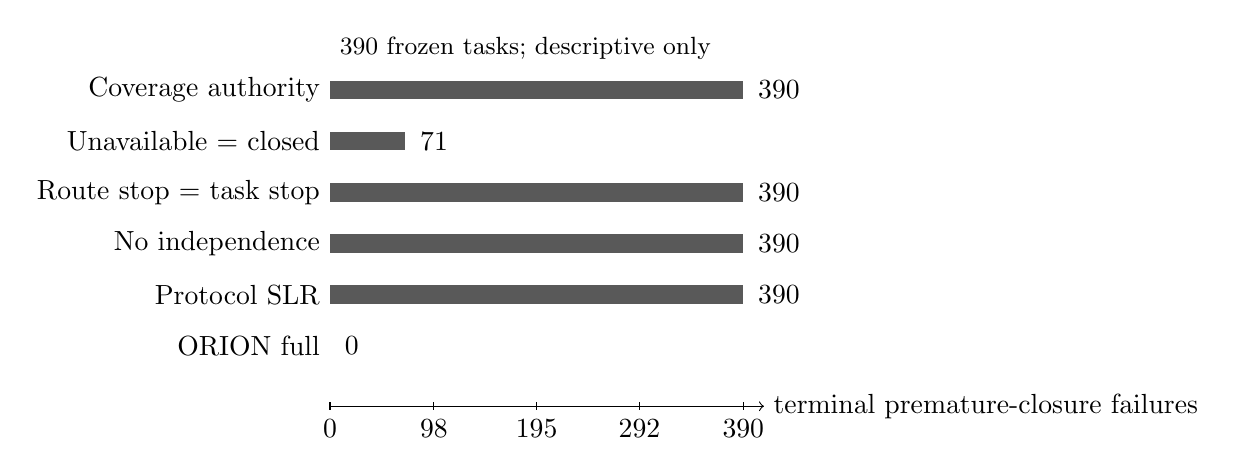
\begin{tikzpicture}[x=0.01346cm,y=0.65cm]
\draw[->] (0,0) -- (409.50,0) node[right]{terminal premature-closure failures};
\draw (0,0.08) -- (0,-0.08) node[below]{0};
\draw (98,0.08) -- (98,-0.08) node[below]{98};
\draw (195,0.08) -- (195,-0.08) node[below]{195};
\draw (292,0.08) -- (292,-0.08) node[below]{292};
\draw (390,0.08) -- (390,-0.08) node[below]{390};
\node[anchor=east] at (-0.35,1.18) {ORION full};
\node[anchor=west] at (4.88,1.18) {0};
\node[anchor=east] at (-0.35,2.18) {Protocol SLR};
\fill[black!65] (0,2) rectangle (390,2.36);
\node[anchor=west] at (394.88,2.18) {390};
\node[anchor=east] at (-0.35,3.18) {No independence};
\fill[black!65] (0,3) rectangle (390,3.36);
\node[anchor=west] at (394.88,3.18) {390};
\node[anchor=east] at (-0.35,4.18) {Route stop $=$ task stop};
\fill[black!65] (0,4) rectangle (390,4.36);
\node[anchor=west] at (394.88,4.18) {390};
\node[anchor=east] at (-0.35,5.18) {Unavailable $=$ closed};
\fill[black!65] (0,5) rectangle (71,5.36);
\node[anchor=west] at (75.88,5.18) {71};
\node[anchor=east] at (-0.35,6.18) {Coverage authority};
\fill[black!65] (0,6) rectangle (390,6.36);
\node[anchor=west] at (394.88,6.18) {390};
\node[anchor=west,font=\small] at (0,7.0) {390 frozen tasks; descriptive only};
\end{tikzpicture}

\caption{Terminal premature-closure classifications for selected control
ablations. Bars are task counts from the frozen complete-gold index, not
inferential estimates. The evaluator uses a fixed failure precedence, so a
displayed terminal class can mask lower-precedence failures.}
\label{fig:p2-6}
\end{figure}

The separate route-stop replay recorded 13 false-positive route stops among
1,950 route-stop events (0.006667). These local errors did not become task-level
false closures because the unresolved route obligation remained open. Among
1,878 task-route instances that reached the evaluator's exhaustion point, no
route-stop false negative was observed. This null result is retained and does
not establish a generally optimal stopping rule.

\subsection{Exact-contract isolation of unresolved-route authority}

The fail-closed controller produced the correct scientific-closure decision in
all 400 protected cases. The donor-complete available-route comparator was
correct on 250 cases, and the global-sufficiency comparator was correct on 100.
The paired difference against the donor-complete comparator was 0.375, with a
95\% domain-stratified bootstrap interval of $[0.3275,0.4225]$. Exact McNemar
discordance was $b=150,c=0$. All 150 comparator errors were the material
unavailable, censored, or provider-invalid cases that its aggregation rule
removed from the denominator.

\begin{table}[t]
\centering
\small
\begin{tabular}{lrrr}
\toprule
Controller & Correct / 400 & False task closures & Clean closure \\
\midrule
Fail-closed control & 400 & 0 & 1.000 \\
Available-route donor product & 250 & 150 & 1.000 \\
Global-sufficiency product & 100 & 300 & 1.000 \\
Information-equivalent product & 400 & 0 & 1.000 \\
\bottomrule
\end{tabular}
\caption{Protected exact-contract battery. The information-equivalent product
receives the same unresolved-route semantics and ties the fail-closed
controller. The result therefore isolates an authority rule rather than
inherent model expressivity or centralization.}
\label{tab:p2-exact-contract}
\end{table}

The nonregression conditions also passed. The fail-closed controller made no
false task closure, closed every clean case correctly, produced no unnecessary
undetermined outcome on clean cases, and made no materiality error on 80
held-out nonmaterial-decoy cases. Performance was identical across the five
acquisition settings. Because the information-equivalent product also achieved
400 correct decisions, the evidence supports the unresolved-route rule only.
It does not support ownership of generic stopping, obligation, or closure
machinery.

\subsection{The registered TREC-COVID gate fails}

BM25 was the best comparator for the registered recall-and-cost decision. Its
mean recall@100 was 0.110334, compared with 0.092642 for the governed
controller. The paired mean difference was $-0.01769$. The point estimate lay
inside the $-0.02$ noninferiority margin, but the 95\% bootstrap interval
$[-0.02729,-0.00906]$ did not. Noninferiority was defined by the interval, so
the recall criterion failed.

The cost criterion also failed. The governed controller read 235.8 candidates
per topic on average, compared with 85.52 for BM25, an increase of 175.7\%
rather than the required 25\% reduction. Its mean route calls were 3.0 rather
than 1.0. The overall registered gate therefore failed on both recall and cost.

\begin{table}[t]
\centering
\small
\begin{tabular}{lrrrr}
\toprule
Arm & recall@100 & nDCG@10 & Mean reads & Mean route calls \\
\midrule
BM25 & 0.110334 & 0.417992 & 85.52 & 1.0 \\
Reciprocal-rank fusion & 0.077365 & 0.489570 & 170.30 & 2.0 \\
Governed controller & 0.092642 & 0.566746 & 235.80 & 3.0 \\
Diagnostic closure variant & 0.092642 & 0.566746 & 235.80 & 3.0 \\
\bottomrule
\end{tabular}
\caption{External TREC-COVID outcomes over 50 paired topics. The registered
decision used recall noninferiority and cost reduction. nDCG@10 was measured but
was not a gate criterion.}
\label{tab:p2-trec}
\end{table}

nDCG@10 moved in the favorable direction. The governed controller exceeded
BM25 by 0.1488, with a 95\% bootstrap interval of $[0.1008,0.1986]$, and won on
42 of 50 topics. This result indicates stronger top-ten ranking quality under
the evaluated arm. It cannot compensate for the failed recall-and-cost gate,
and no threshold or endpoint was changed after observing it.

\subsection{External stress-test boundaries}

The MetaSyn probe completed all 86 released test reviews. Macro retrieval
recall was 0.7485 and final inclusion recall was 0.5651. Of 1,677 reference
links, 598 were absent from the retrieved pools and another 343 were lost during
screening, leaving 941 final false negatives. This result attributes loss
within a bounded retrieval-and-screening probe; it does not evaluate the full
controller.

\begin{table}[t]
\centering
\small
\begin{tabular}{>{\raggedright\arraybackslash}p{0.23\linewidth}>{\raggedright\arraybackslash}p{0.36\linewidth}>{\raggedright\arraybackslash}p{0.32\linewidth}}
\toprule
Evidence family & Observed result & Allowed interpretation \\
\midrule
MetaSyn public probe & Retrieval recall 0.7485; inclusion recall 0.5651 &
Bounded stage attribution only \\
AutoResearchBench Deep & 0/600 title matches after a 9/9 judge control &
Bounded negative candidate-generation diagnostic \\
OpenAIRE/Crossref & Provider validity below the frozen 0.90 threshold &
Comparison remains undetermined; zero differences are not equivalence \\
Public screening transport & Frozen donor outperforms the candidate on primary
recall and work-saving endpoints in multiple development studies &
Adverse within-pool evidence; not an acquisition or closure test \\
\bottomrule
\end{tabular}
\caption{External results retained at separate authority levels. No row is
averaged with the TREC-COVID decision or promoted into system superiority.}
\label{tab:p2-external-boundaries}
\end{table}

The AutoResearchBench Deep probe returned no official title match across 600
tasks after its positive and negative judge control passed all nine cases. A
separate stage analysis found negligible exact and substring recovery in the
candidate sets, making candidate generation rather than the judge the bounded
failure location. The result is not a matched baseline comparison.

The matched OpenAIRE/Crossref campaigns failed provider-validity thresholds.
Their observed paired differences were zero because retrieval operated near a
measurement floor or the route transport was invalid. Resampling identical
near-zero differences yields a narrow interval regardless of scientific
informativeness, so no equivalence or noninferiority conclusion is drawn. These
undetermined outcomes and the adverse public screening results remain visible
as limits on external generalization.
